%\chapter{System presentation}
%Aalborg University has provided the project group with a pre-built mini segway. Based on the system design of an segway this chapter will, present and describe the mini segway, with a focus on the mechanical frame and the provided hardware. 
\section{Description of Provided Segway} \label{sec:hardware}
Before the modelling and the design of the controller can begin, the segway provided by the university first has to be described, especially in regards to the electronic hardware used on the segway. This is done in the following section. A photo of the provided segway can be seen in \autoref{hardwarePlatform}. 

\begin{figure}[H]
	\centering
	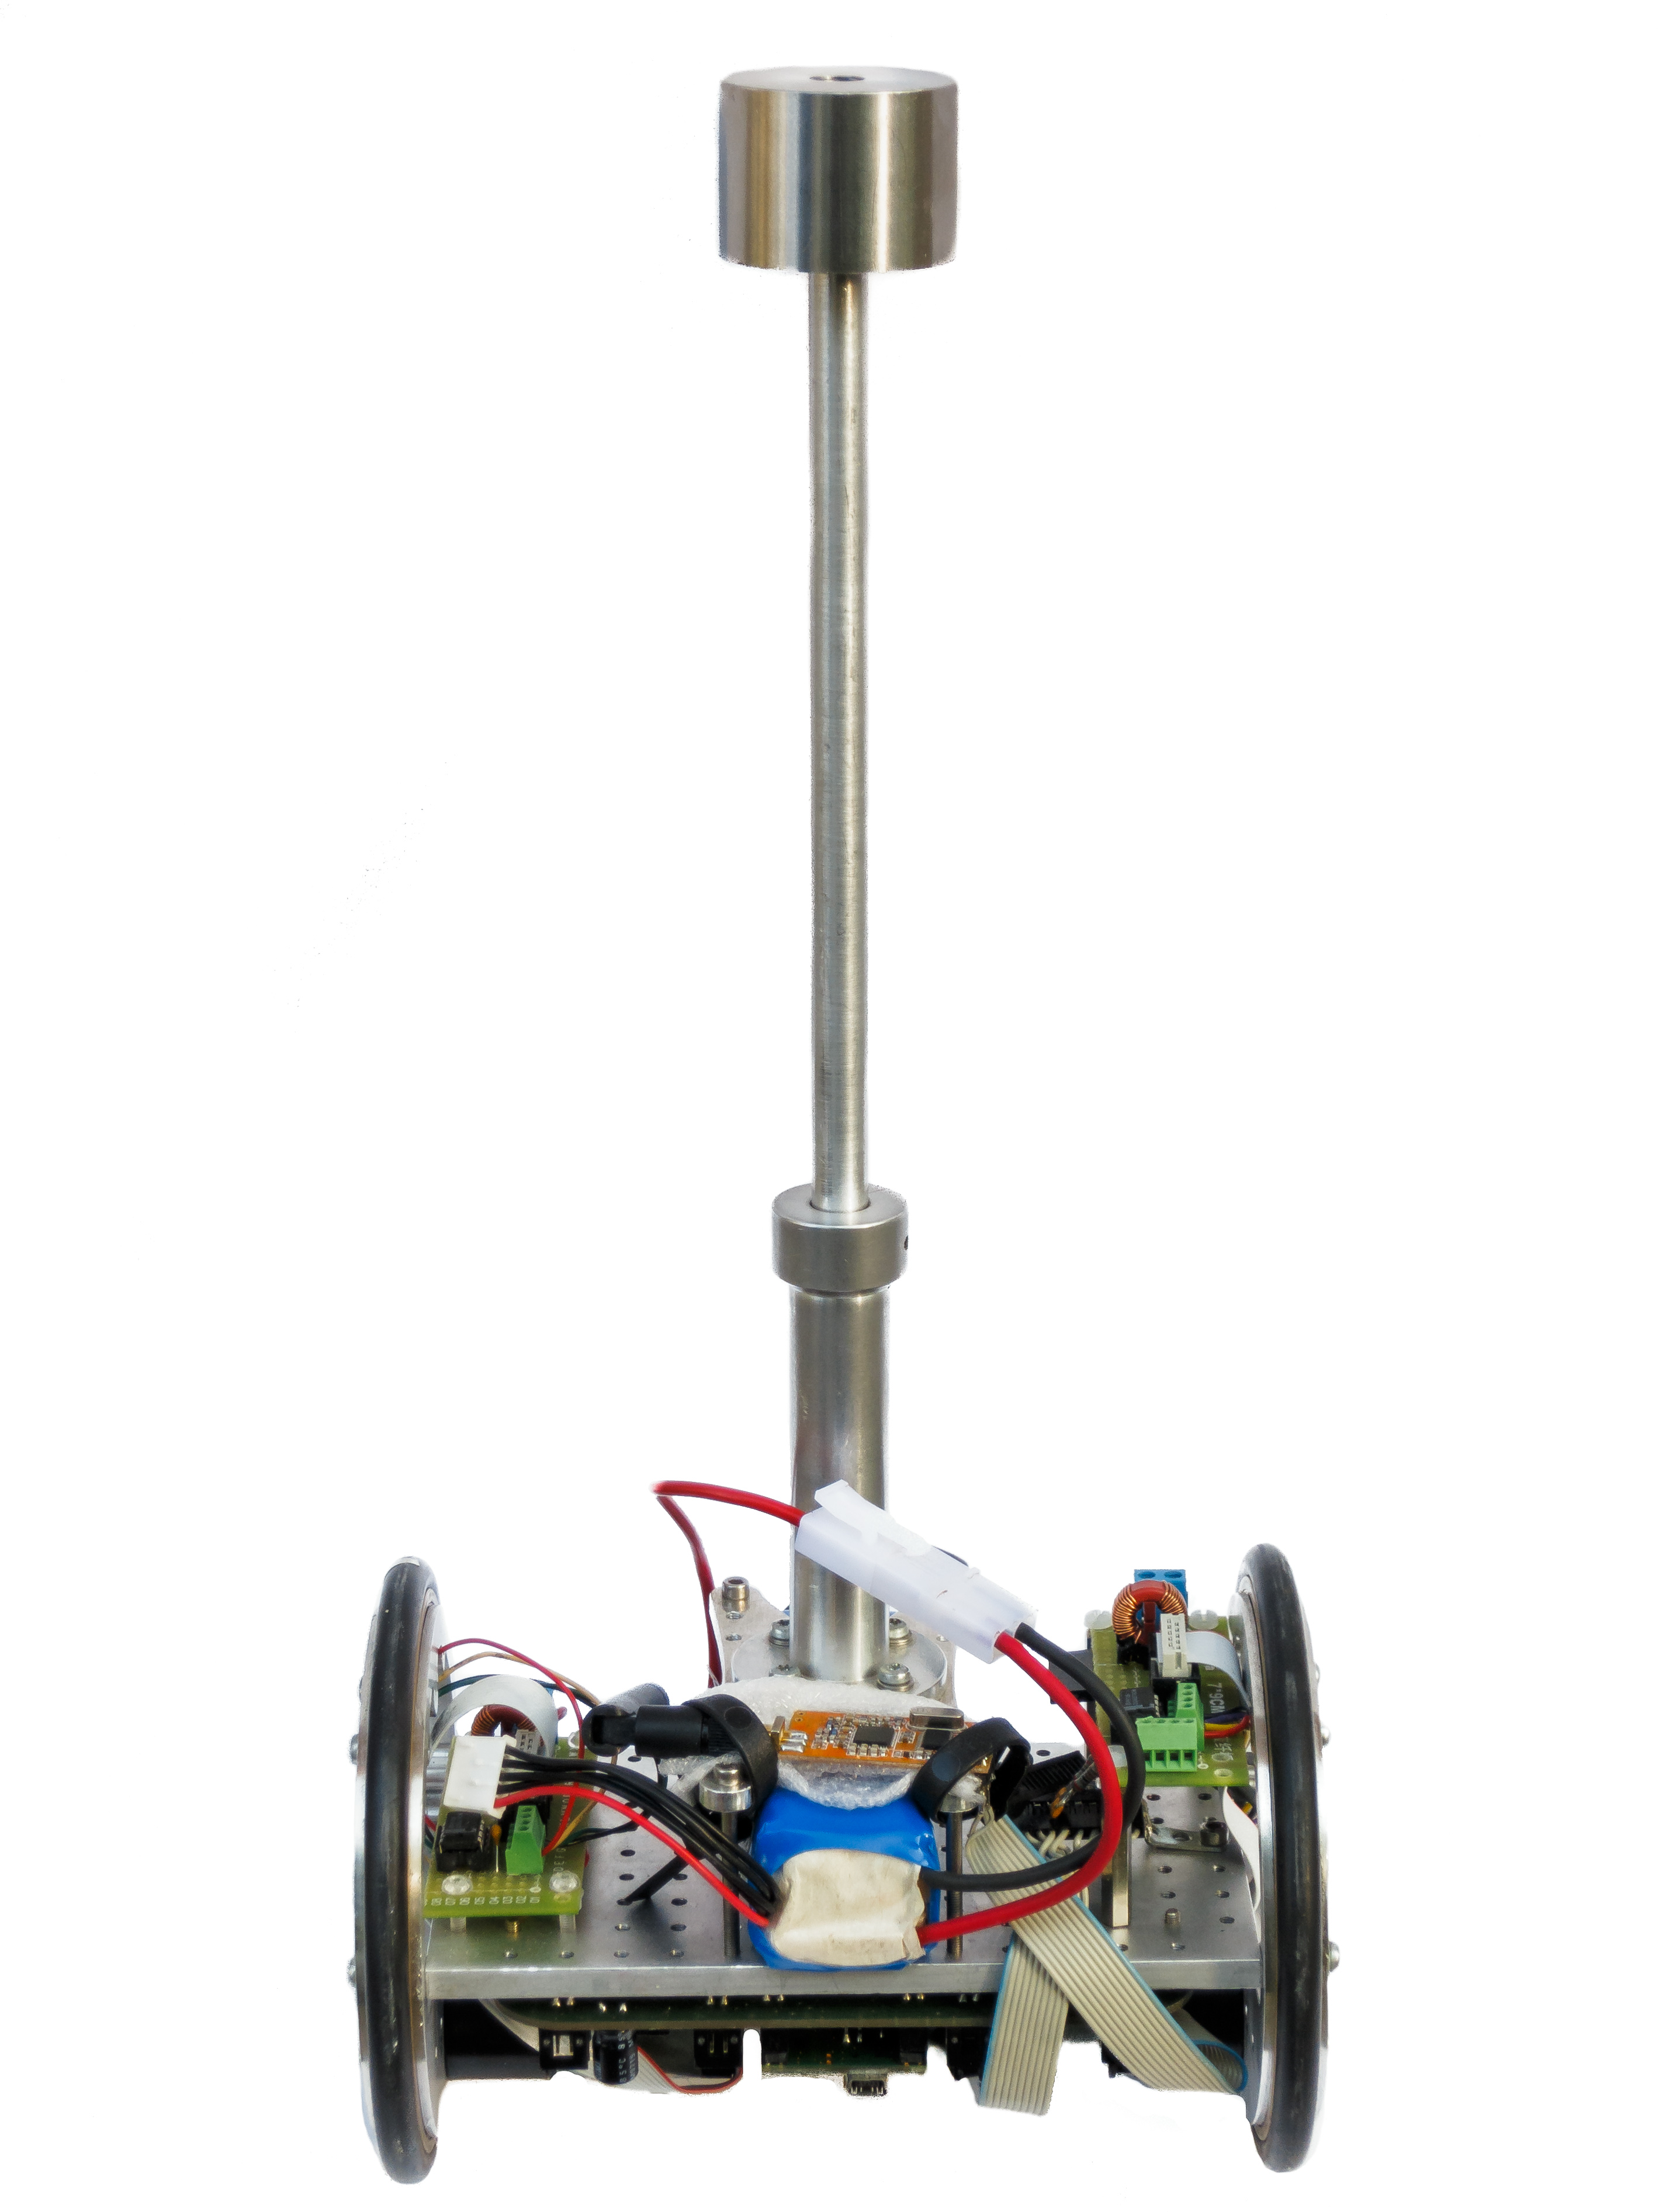
\includegraphics[width=0.4\textwidth]{figures/hardwarePlatform.jpg}
	\caption{The segway to be used in the project.}
	\label{hardwarePlatform}
\end{figure}

The segway consists of several items, these items are divided into 3 main groups, namely \textbf{mechanical}, \textbf{power} and \textbf{electronics}. These groups and the items they include are described in the following.

%\begin{itemize}
%
%\item \textbf{Mechanical}
%\begin{itemize}
%\item Mechanical frame
%\item Wheels
%\item Motors
%\end{itemize}
%
%\item \textbf{Power}
%\begin{itemize}
%\item Batteries
%\item PSUs (Power Supply Units)
%\end{itemize}
%
%\item \textbf{Electronics}
%\begin{itemize}
%\item Wireless transceivers
%\item Microcontroller
%\item Filters
%\item Accelerometer + gyroscope
%\item Motor driver
%\item Encoders
%\end{itemize}

%\end{itemize}
%\todo{remove list, write as text}
%These will be described in further details in the following.

\subsection{Mechanicanics}
\subsubsection{Mechanical Frame}

The provided segway's mechanical frame is made from aluminium. It consists of a baseplate onto which the wheels are mounted, together with a rod with a cylindrical mass on top. All electronics including batteries are mounted on the baseplate.

A blueprint of the segway can be seen in \autoref{segwaySchematic} in \appref{app:segwayParameters}, and measurements of relevant parameters of the frame is listed in \autoref{tab:dimensions}, also in \appref{app:segwayParameters}.


%\begin{wrapfigure}{R}{0.5\textwidth}
%\centering
%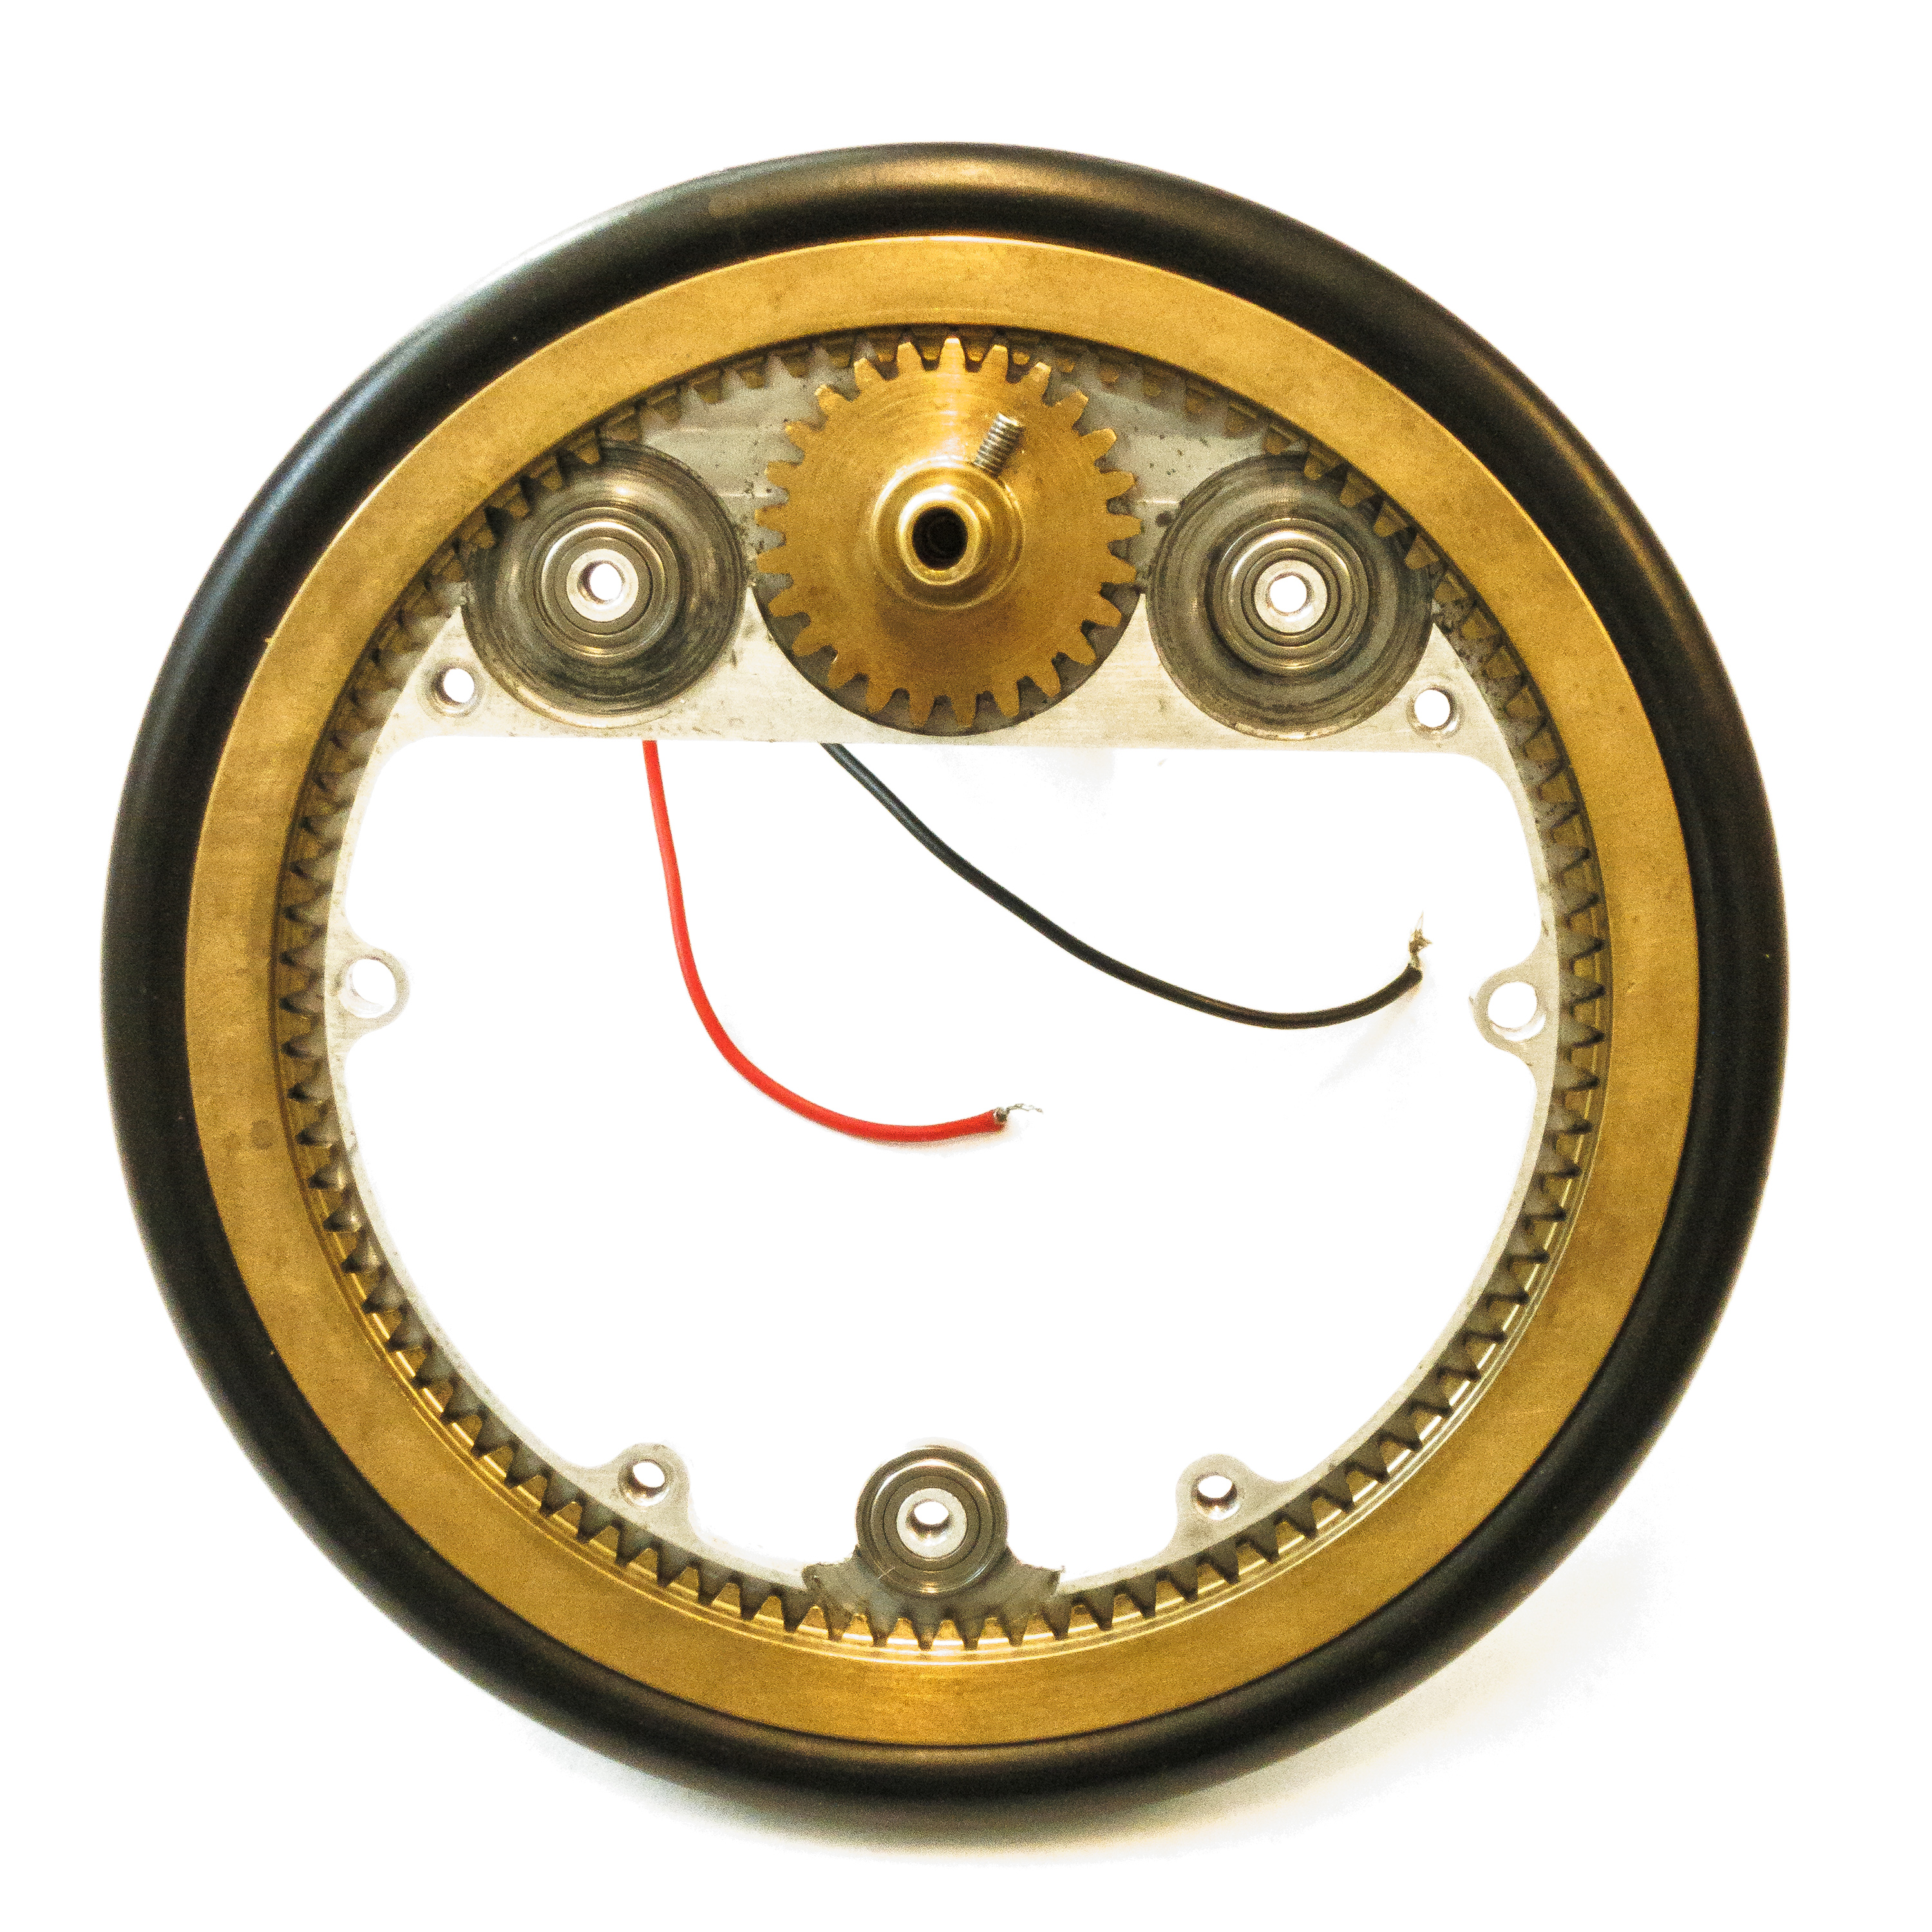
\includegraphics[width=0.4\textwidth]{figures/wheel.jpg}
%\caption{The wheel and motor showing the transmission(motor behind the small gear)}
%\label{fig:wheel}
% \vspace{-4cm}
%\end{wrapfigure}


\subsubsection{Wheels}
\label{subsec:wheels}
The wheels mounted on the segway feature an offset motor, meaning the motor is not mounted at the center. Though, as seen from the blueprint in \autoref{segwaySchematic} in \appref{app:segwayParameters}, the axis of the wheel is still in the center of the base. The wheel system is built as follows: The motor rotates a gear fitted onto the motor from the factory. The shaft from this gear is located on the inner side of the wheel, and mounted to a cogwheel. The inner side of the wheel itself has some small cogs making it the other part of the transmission system.
For a better rotation and less friction, the wheel has three ball bearing guides. This can be seen in \autoref{fig:wheel}.
The cogwheel mounted on the motor wheel has 25 cogs and the inside of the wheel has 90 cogs.

\begin{figure}[H]
\centering
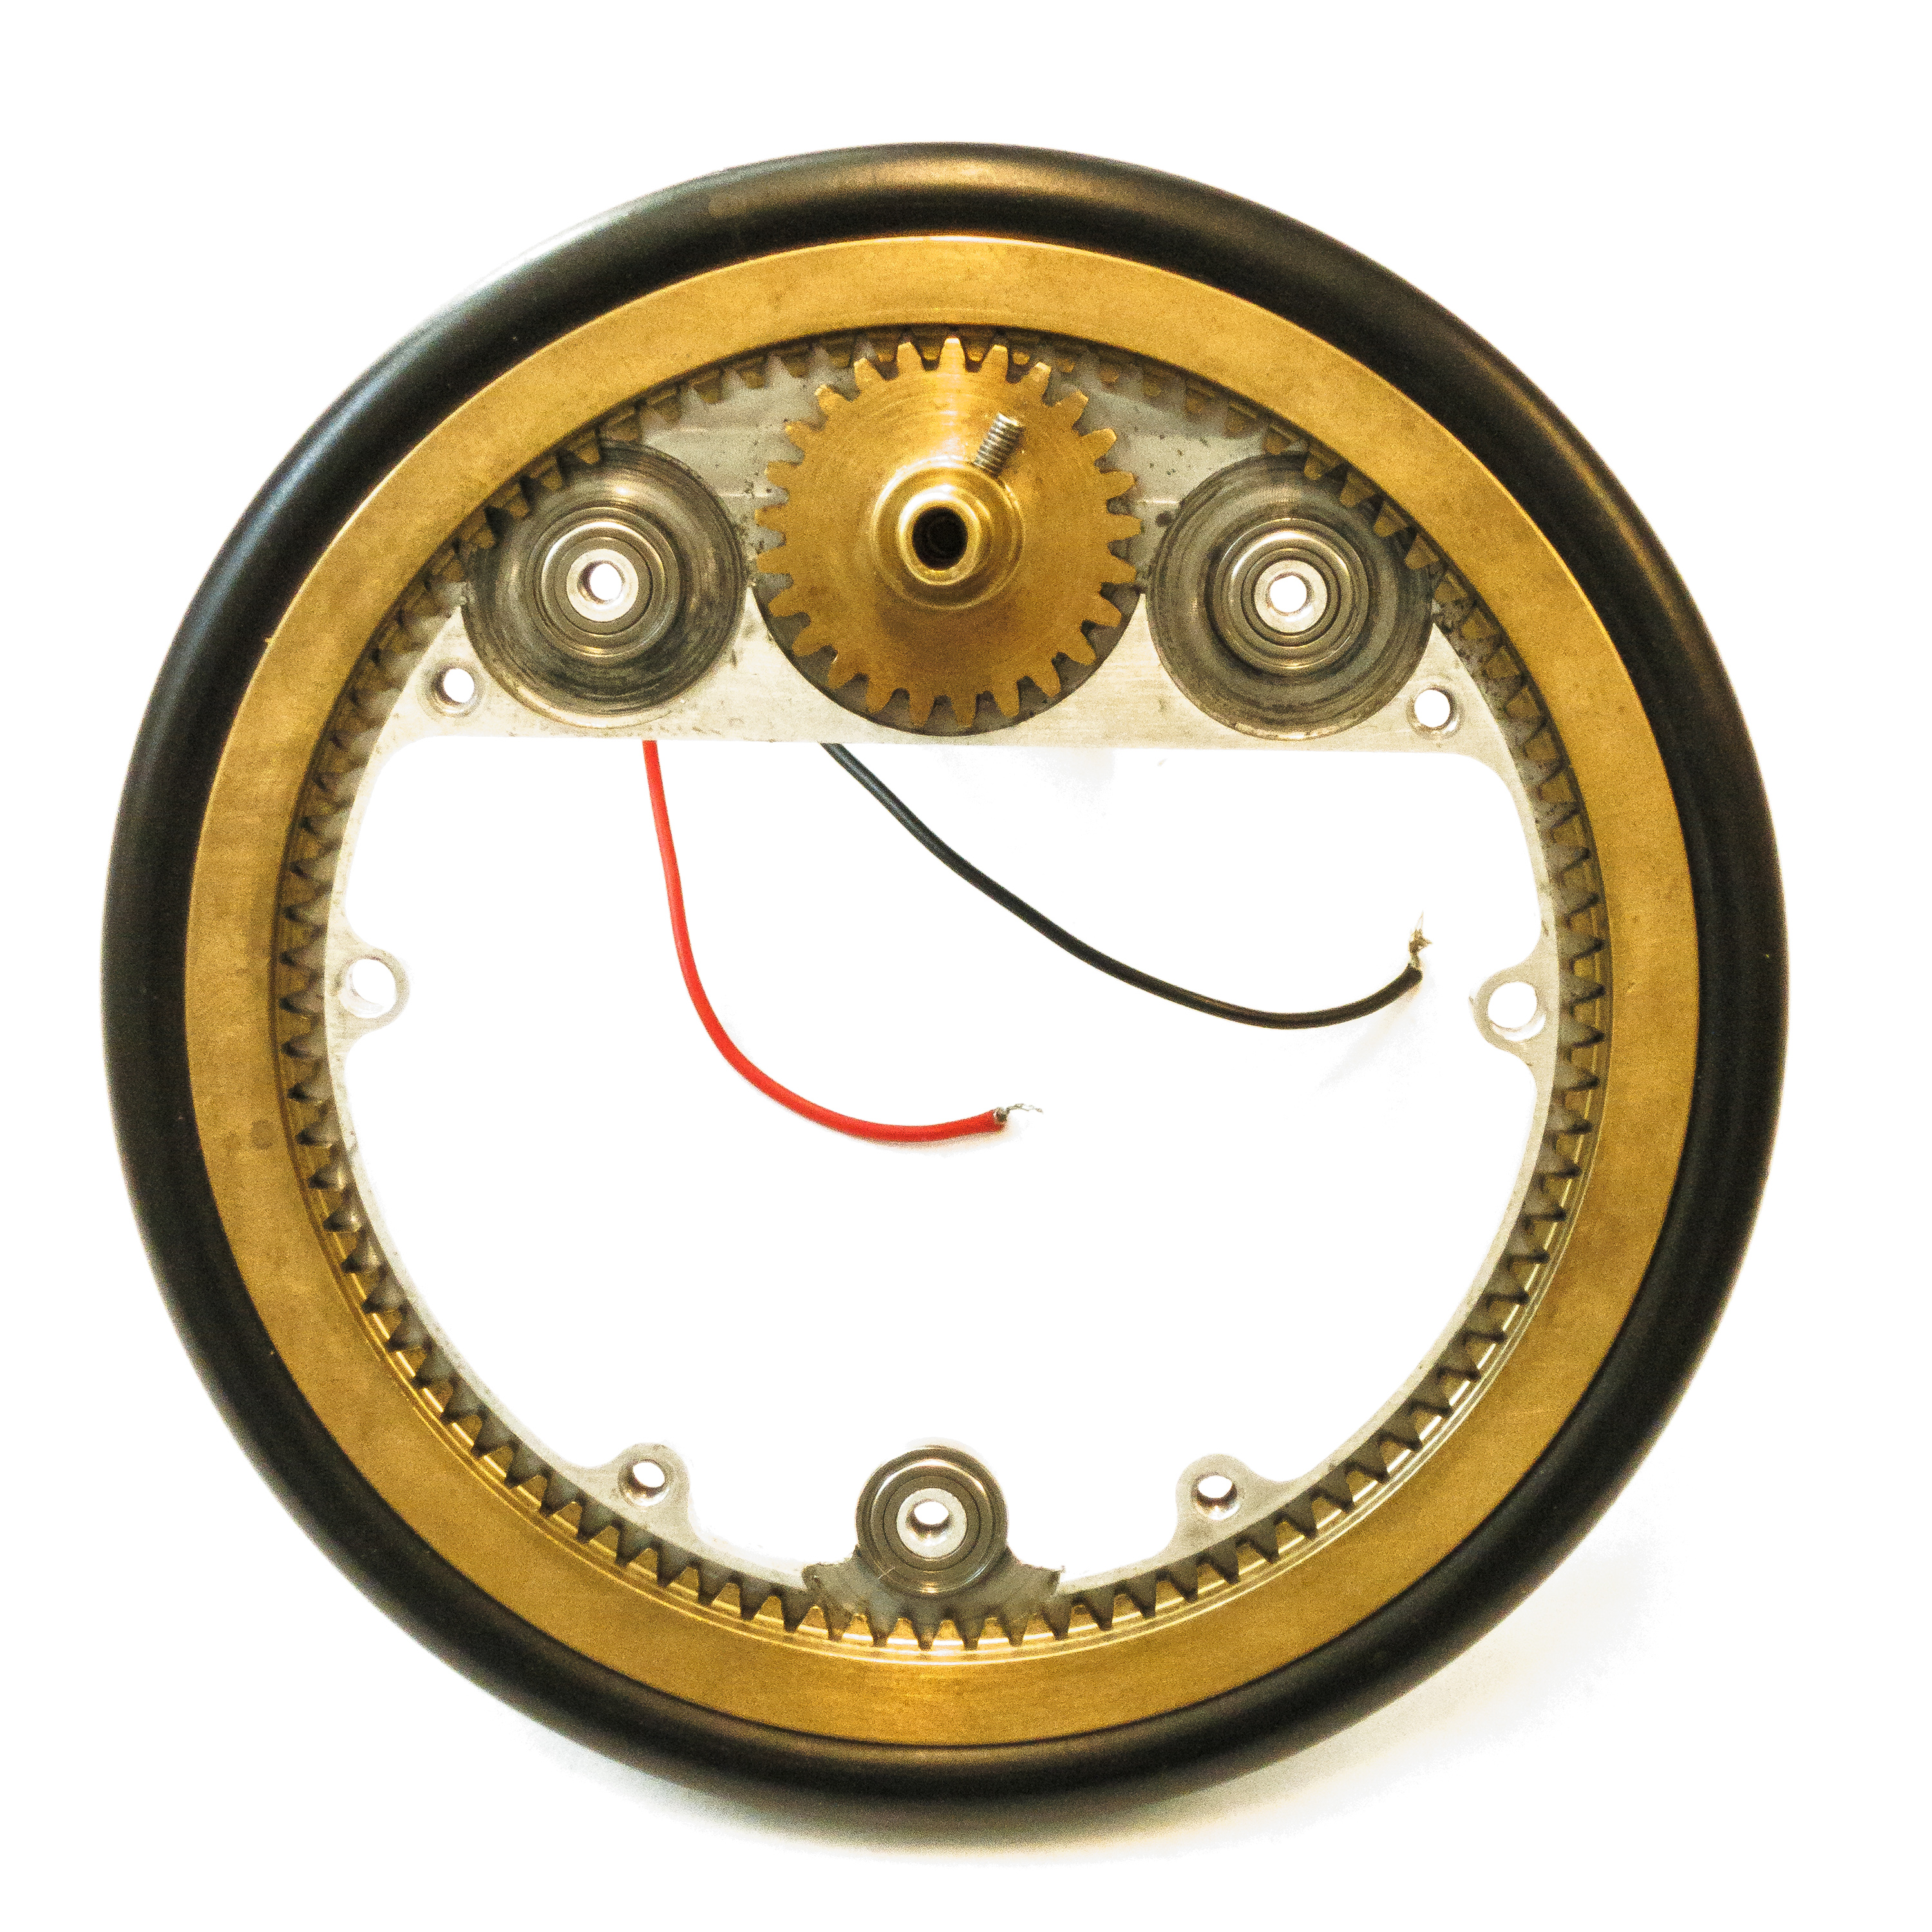
\includegraphics[width=0.4\textwidth]{figures/wheel.jpg}
\caption{The wheel and motor showing the transmission. The motor is behind the small gear.}
\label{fig:wheel}
\end{figure}

\subsubsection{Motors}
\label{subsec:motors}
The segway uses two Maxon A-Max 110160 permanent DC-motors to rotate the wheels. Parameters of the motors that might be taken into account are the rotational speed and the torque. The specification of the motors are \citep{maxon}
\begin{itemize}
\item Nominal torque at {6 V} is 5.91 mNm.
\item Nominal speed at {6 V} is 6240 RPM.
\end{itemize}

%A permanent DC motor is working by rotating an armature within a magnetic field. This produces a mechanical force, when a current carrying conductor is placed in the magnetic field, as this is exerting an equal and opposite force due to Newton's third law. 

%The rotational speed is given in RPM (Revolutions Per Minute) and the torque is given in mNm (milli Newton meter).

The motors are brushed, meaning the stator corresponds to the magnets and the rotor is composed of the coils, receiving power through brushes.
Brushed motors have important advantages: They have a low cost of construction, require only simple and inexpensive control and they operate in extreme environments due to lack of electronics. However, those motors also have drawbacks: They require periodic maintenance, their characteristics are moderately flat and at high speeds, brush friction increases, thus reducing useful torque. Also, the brush arcing will generate noise causing electrical magnetic interference (EMI) \citep{BvsBL} \citep{BvsBLv2}.

\begin{figure}[H]
	\centering
	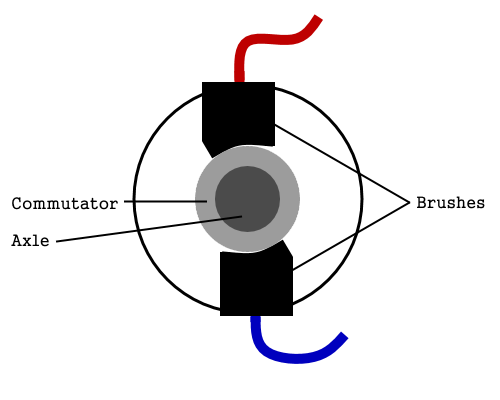
\includegraphics[width=0.5\textwidth]{figures/brushed_2.png}
	\caption{Sectional view of a brushed motors.}
	\label{DCBrushed}
\end{figure}

As a part of the motors, a gear (Maxon 110356) has been fitted on the motor. This gear was fitted from the factory, and the inner workings of it are therefore not known. From the datasheet, the gear ratio between the motor and shaft is known \citep{gear}: 
$$N_{ms} = \frac{1}{19} \approx 0.053$$

\subsection{Power}
\subsubsection{Batteries}
The segway comes equipped with a battery which is the source of power of the system. The battery is a rechargeable 4S LiPo. LiPo batteries, or Lithium-ion Polymer batteries, consists of cells in series, \textit{x}S meaning \textbf{\textit{x}} cells in \textbf{S}eries. A LiPo cell has a nominal voltage of 3.7V. The battery used on the device has a nominal voltage of 14.8 V (3.7 Volts times 4 cells).
LiPo batteries, compared to other types such as Nickel–metal hydride (NiMH), one of the most common battery types, are lighter and more compact. However, they are more expensive than "regular" batteries and require a specific charger to bring every cell of the pack to the same state of charge \citep{Cells}.

The Segway also has two Power Supply Units (PSU's). These are electronic components, whose role it is to regulate the unstable input voltage from the batteries, to a stable voltage to be used by the electronics.
One has an output of 5V and the other has an output of 3.3V. 

\pagebreak 
\subsection{Electronics}
\subsubsection{Wireless Transceivers}
To facilitate the wireless communication between the segway and a remote controller, a pair of APC220 radio communication modules is supplied.
The modules have the following features \citep{wifimodule}:
\begin{itemize}
\item Transmission distance of up to 1000 m (2400 baud)
\item UART/TTL interface with 256 bytes data buffer
\item -112 dBm sensitivity at 9600 baud
\item 20 mW output power
\item Adjustable frequency from 418 MHz to 455 MHz
\end{itemize}

Since the modules have a UART interface, they can be interfaced through a UART interface on a microcontroller, which makes the radio modules simple and easy to use.

\subsubsection{Microcontroller}

A microcontroller board is supplied with the segway. The \gls{PCB} on which all the electrical components are mounted, is designed to fit the supplied \gls{MCU}, and thus a new MCU is not chosen, since it might require a redesign of the PCB.

The microcontroller board supplied is a \emph{CrumbX128A3} made by Chip45 \citep{CrumbX128A3}. The CrumbX128A3 features an ATxmega128A3U microcontroller, a 3.3V low dropout (LDO) voltage regulator, a USB UART converter, an RS485 transceiver and a micro-sd-card header/slot.
	
The ATxmega128A3U has the following specifications \citep{xmega}:

\begin{itemize}
\item 32 MHz clock speed
\item $1.6-3.6$ V power supply
\item 128 Kb flash
\item 8 KB SRAM
\item 7 UARTs
\item 7 16-bit counters
\item 4-channel DMA controller
\end{itemize}
\subsubsection{Accelerometer and Gyroscope}
To measure the angle the segway is tilted as well as its relative position, an accelerometer and gyroscope is used. Here, the InvenSense MPU-6050\citep{gyro} is used, a 6-axis gyroscope and accelerometer. The chip is implemented on a GY-521 breakout board. It features an \iic bus, from which the raw sensor values can be read. 
The gyroscope can be configured to having a full-scale range of either $\pm 250, \pm 500, \pm 1000$ or $\pm 2000 \degree /\text{sec}$. The accelerometer can be programmed to have a full-scale range of $\pm 2g, \pm 4g, \pm 8g$ or $\pm 16g$ \citep{gyro}.

\subsubsection{Motor Driver}
To control the motors, a motor driver is used, in form of an H-bridge. The H-bridge allows a small controller-voltage to control a (often relatively large) current. This is practical, since the current needed to drive most motors is bigger than what can be drawn from the pins of a microcontroller. 
Here, two Freescale MC33926 5A H-bridges \citep{hbridge} are supplied - one for each motor. The H-bridge makes it possible for a motor to be run both forward and backwards, based on the input signals to the chip. It also features a feedback-pin, also known as a current sense, that can be used to measure the current drawn by the motor. The H-bridge is controlled by an input PWM signal and two direction pins. By setting these pins, the motor can be either locked, free-running or moving forwards or backwards.

\subsubsection{Encoders}\label{subsec:preEncoder}
In order to keep the inverted pendulum in balance, the segway needs a way to quantify the amount of rotation on the wheels and, by extension, on the motors, hence the encoders. The ones currently used by the system are relative (or incremental) encoders placed directly on the motors.
An incremental encoder delivers a certain number of pulses per revolution. This number of pulses measures the angular movement.
Usually, relative encoders consist of a disc divided in transparent and opaque segments. Most of those discs are equipped with two rows of segments plus a top segment. Both segment tracks are slightly out of phase to indicate the direction of rotation and the additional top segment allows the count of revolutions.
An incremental encoder's resolution corresponds to the maximum number of pulses sent per revolution and is symbolised by the unit "points per rotation" \citep{IncEnc}.
\vspace{-1 cm}
\begin{figure}[H]
	\centering
	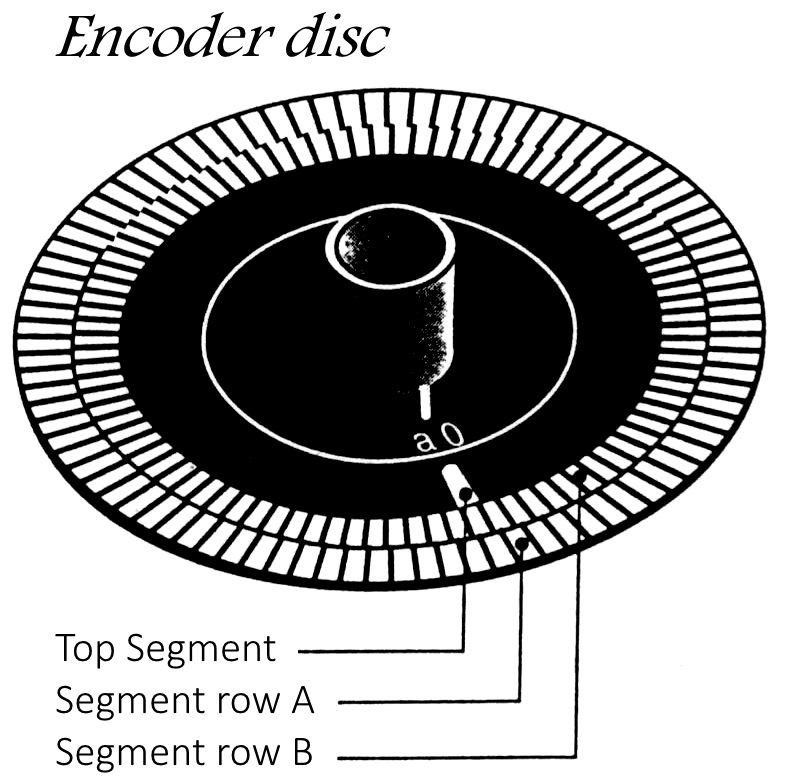
\includegraphics[width=0.36\textwidth]{figures/Encoder.jpg}
	\caption{Detailed scheme of an incremental encoder \citep{IncEnc}.}
	\label{fig:incremental_encoders}
\end{figure}

%Placed between the motor encoders and the microcontroller, are some filters. The filter type used is not known, nor is the filter specifications. Since its inputs and outputs are unknown, it is considered a black box.
%Because of this, it is decided to remove these filters and design new filters, so the exact transfer function of them is known.

\newpage
\subsection{Detailed Segway Overview}
The general block diagram of the segway control system in \autoref{fig:seg_over} can be extended based on the provided hardware described above. The detailed diagram can be seen in \autoref{fig:ext_seg_over}.

\begin{figure}[H]
\centering
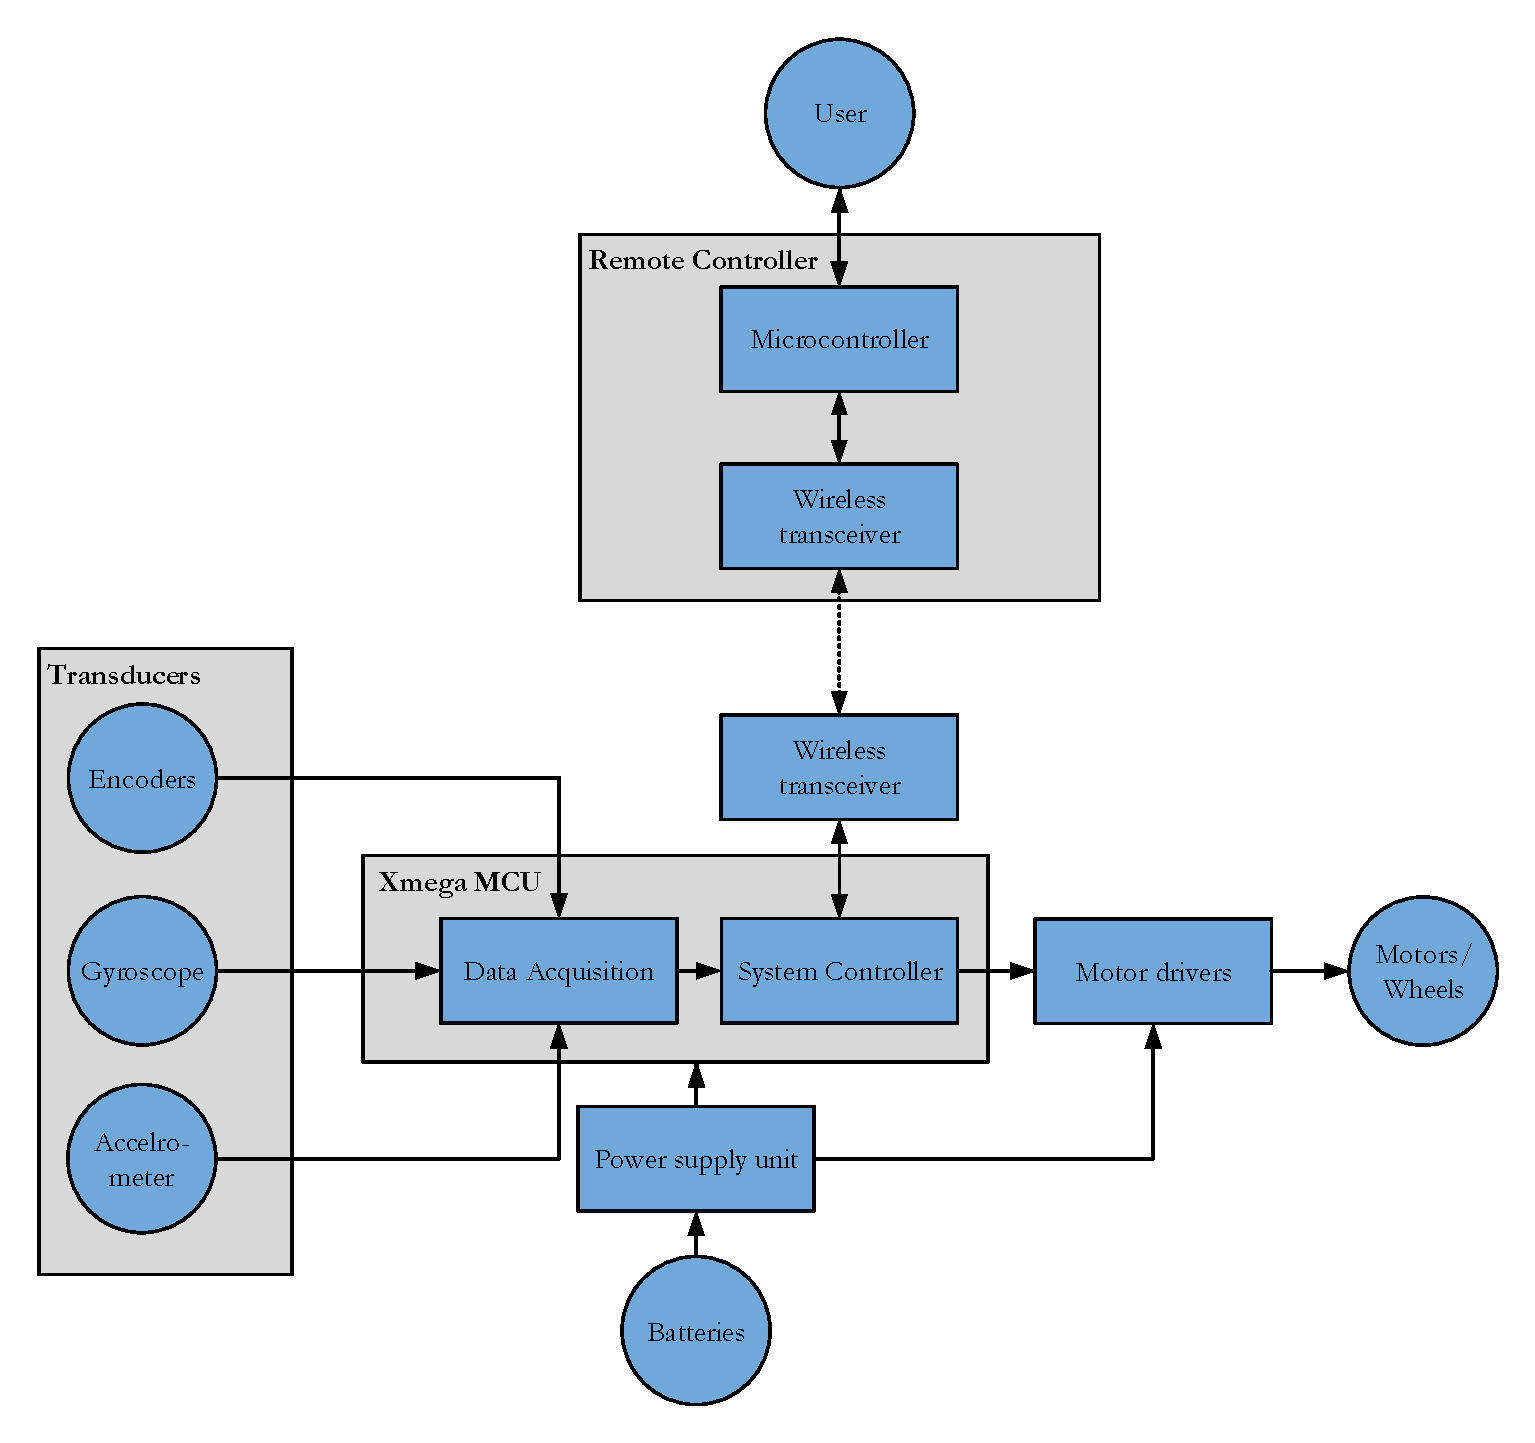
\includegraphics[width = 0.95\textwidth]{figures/extendedOverview.pdf}
\caption{Detailed block diagram of the segway system.}
\label{fig:ext_seg_over}
\end{figure}

In the detailed diagram, the different transducers have been added, and the functionalities the MCU is to facilitate have been grouped. Also, the actuator has been specified, in the form of motors.
The workings of the remote controller are also described in further details, namely that it is to receive user input to a MCU and then transmit it wirelessly. It can also display data from the segway to the user. Also added to \autoref{fig:ext_seg_over} are the batteries and PSUs. 

